%!TEX root = supplement.tex

%%%%%%%%%%%%%%%%%%%
\begin{figure}
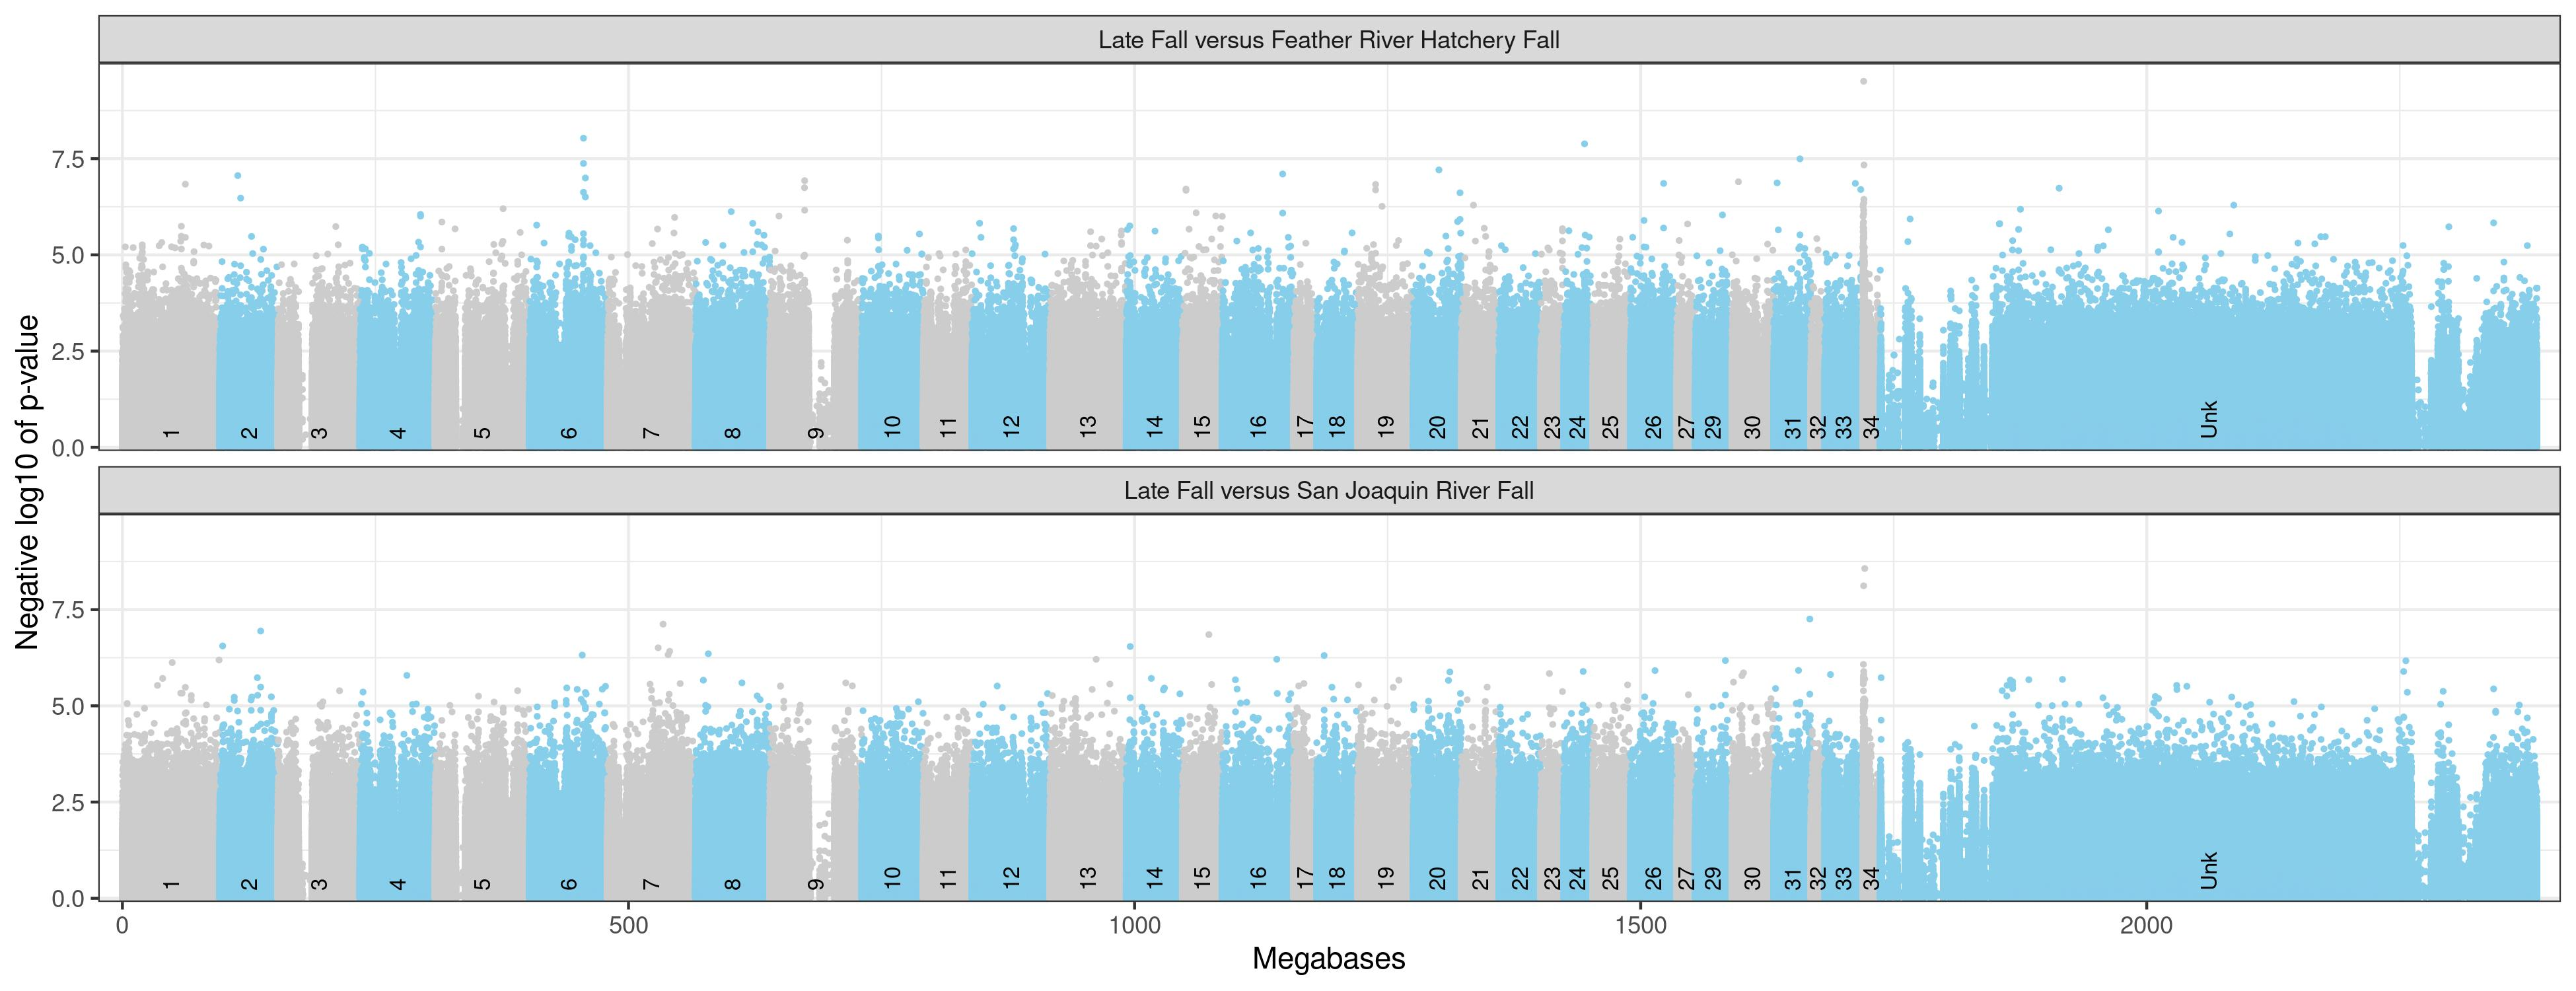
\includegraphics[width=\textwidth]{images/lfar-assoc-faceted.jpg}
\caption[
	Negative log base 10 of association $p$-values for
	individual SNPs for late-fall versus fall run
]{
	\footnotesize Negative log base 10 of association $p$-values for
	individual SNPs for late-fall versus fall run.  $x$ axis shows position in genome (in megabases),
	with color alternating by chromosome, as indicated by numbers above the $x$-axis. ``Unk'' refers
	to unplaced scaffolds in the Otsh\_v1.0 genome assembly \citep{christensen2018chinook}. The 
	upper panel is the comparison between late-fall and Feather River Hatchery fall, while the lower 
	panel is the comparison of late-fall to San Joaquin River fall. 
}
\label{fig:lfar-assoc}
\end{figure}



%%%%%%%%%%%%%%%%%%%%%% 
\begin{figure}
\begin{center}
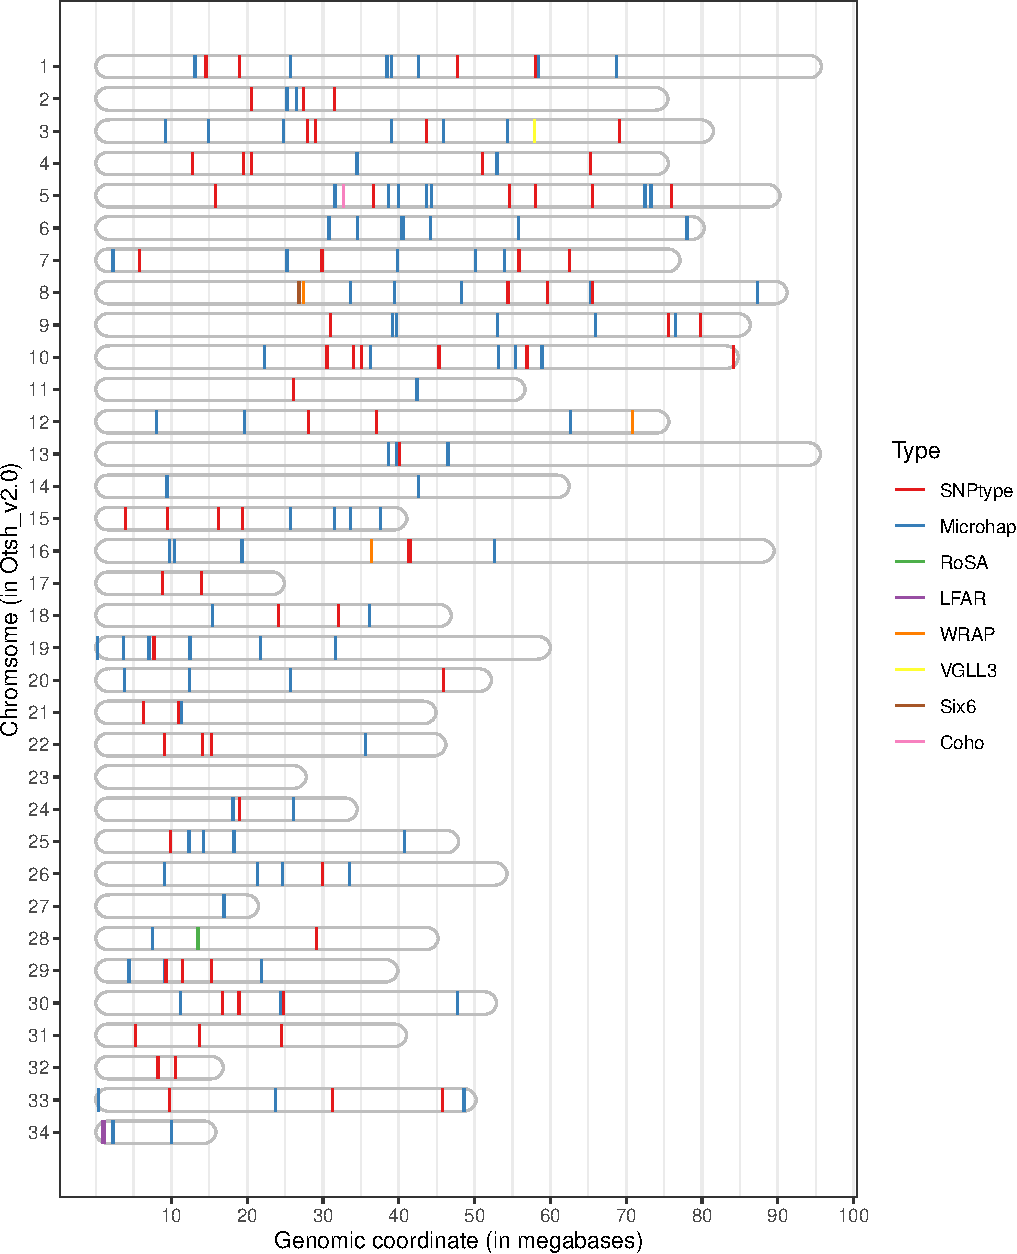
\includegraphics[width=0.7\textwidth]{images/genomic-locations-plot.pdf}
\end{center}
\caption[Genomic locations of amplicons]{\footnotesize Genomic locations of amplicons in the
Otsh\_v2.0 assembly of the Chinook salmon genome.  Color shows type of marker (see main text).
The sex-ID marker is not included here because it aligns to a scaffold that is not part of a
named chromosome/linkage group in the assembly.}
\label{fig:num-alle}
\end{figure}
%%%%%%%%%%%%%%%%%%%%





%%%%%%%%%%%%%%%%%%%%%% 
\begin{figure}
\begin{center}
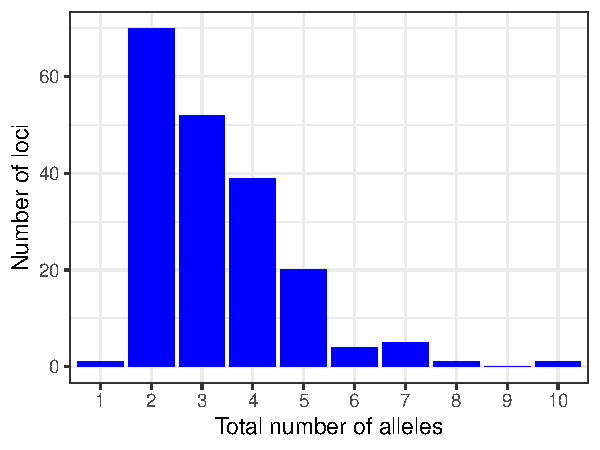
\includegraphics[width=0.7\textwidth]{images/num-alle-barplot.pdf}
\end{center}
\caption[Number of loci with different
total numbers of alleles]{\footnotesize Number of loci with different
total numbers of alleles in the data set. The one amplicon with only
one allele is {\tt Ots\_coho001\_05\_32691399}, which is fixed for alternate alleles
in Chinook vs.\ coho salmon. It is helpful in identifying coho samples that are
misidentified during sampling as Chinook salmon.}
\label{fig:num-alle}
\end{figure}
%%%%%%%%%%%%%%%%%%%%




%%%%%%%%%%%%%%%%%%%%%% 
\begin{figure}
\begin{center}
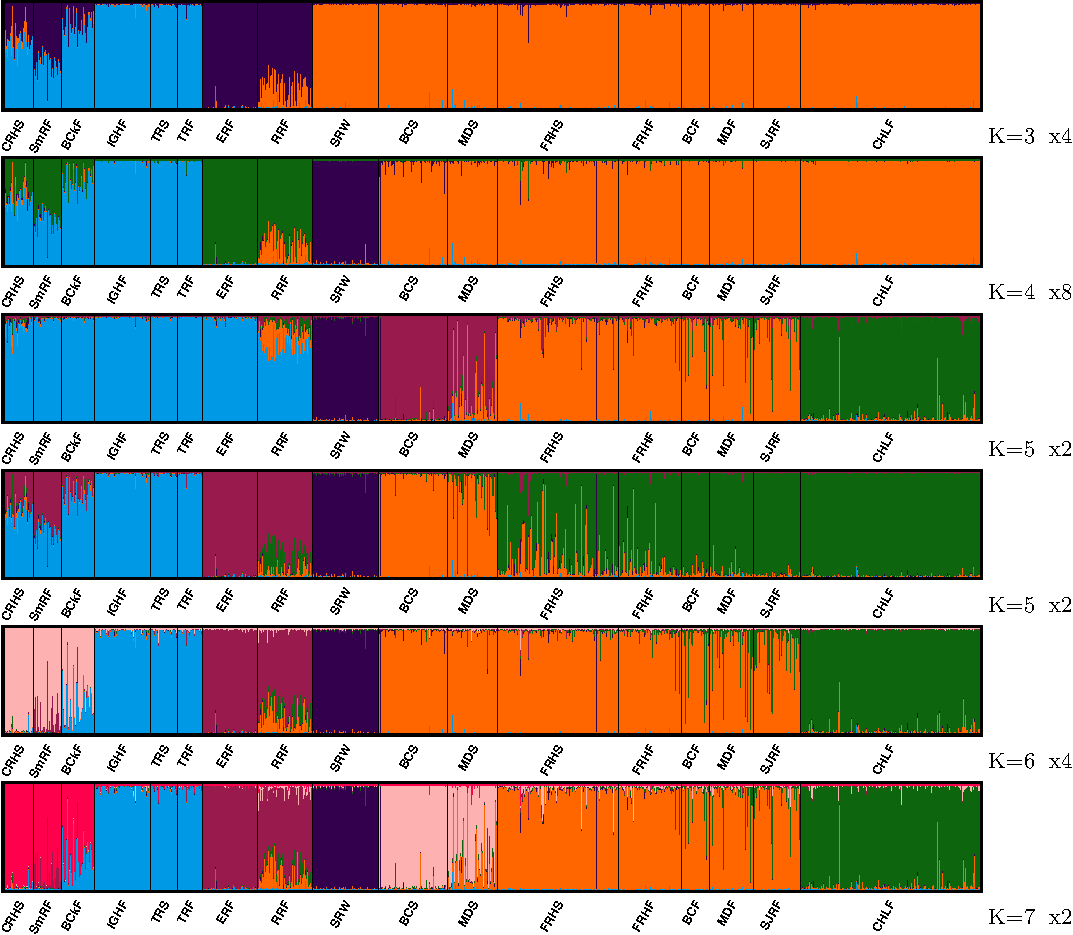
\includegraphics[width=0.7\textwidth]{images/minor-modes-crop.pdf}
\end{center}
\caption[STRUCTURE minor modes found by CLUMPAK]{\footnotesize At each value of $K$
for which a minor mode was found, these plots show them}
\label{fig:minor-modes}
\end{figure}
%%%%%%%%%%%%%%%%%%%%


%%%%%%%%%%%%%%%%%%%%%% 
\begin{figure}
\begin{center}
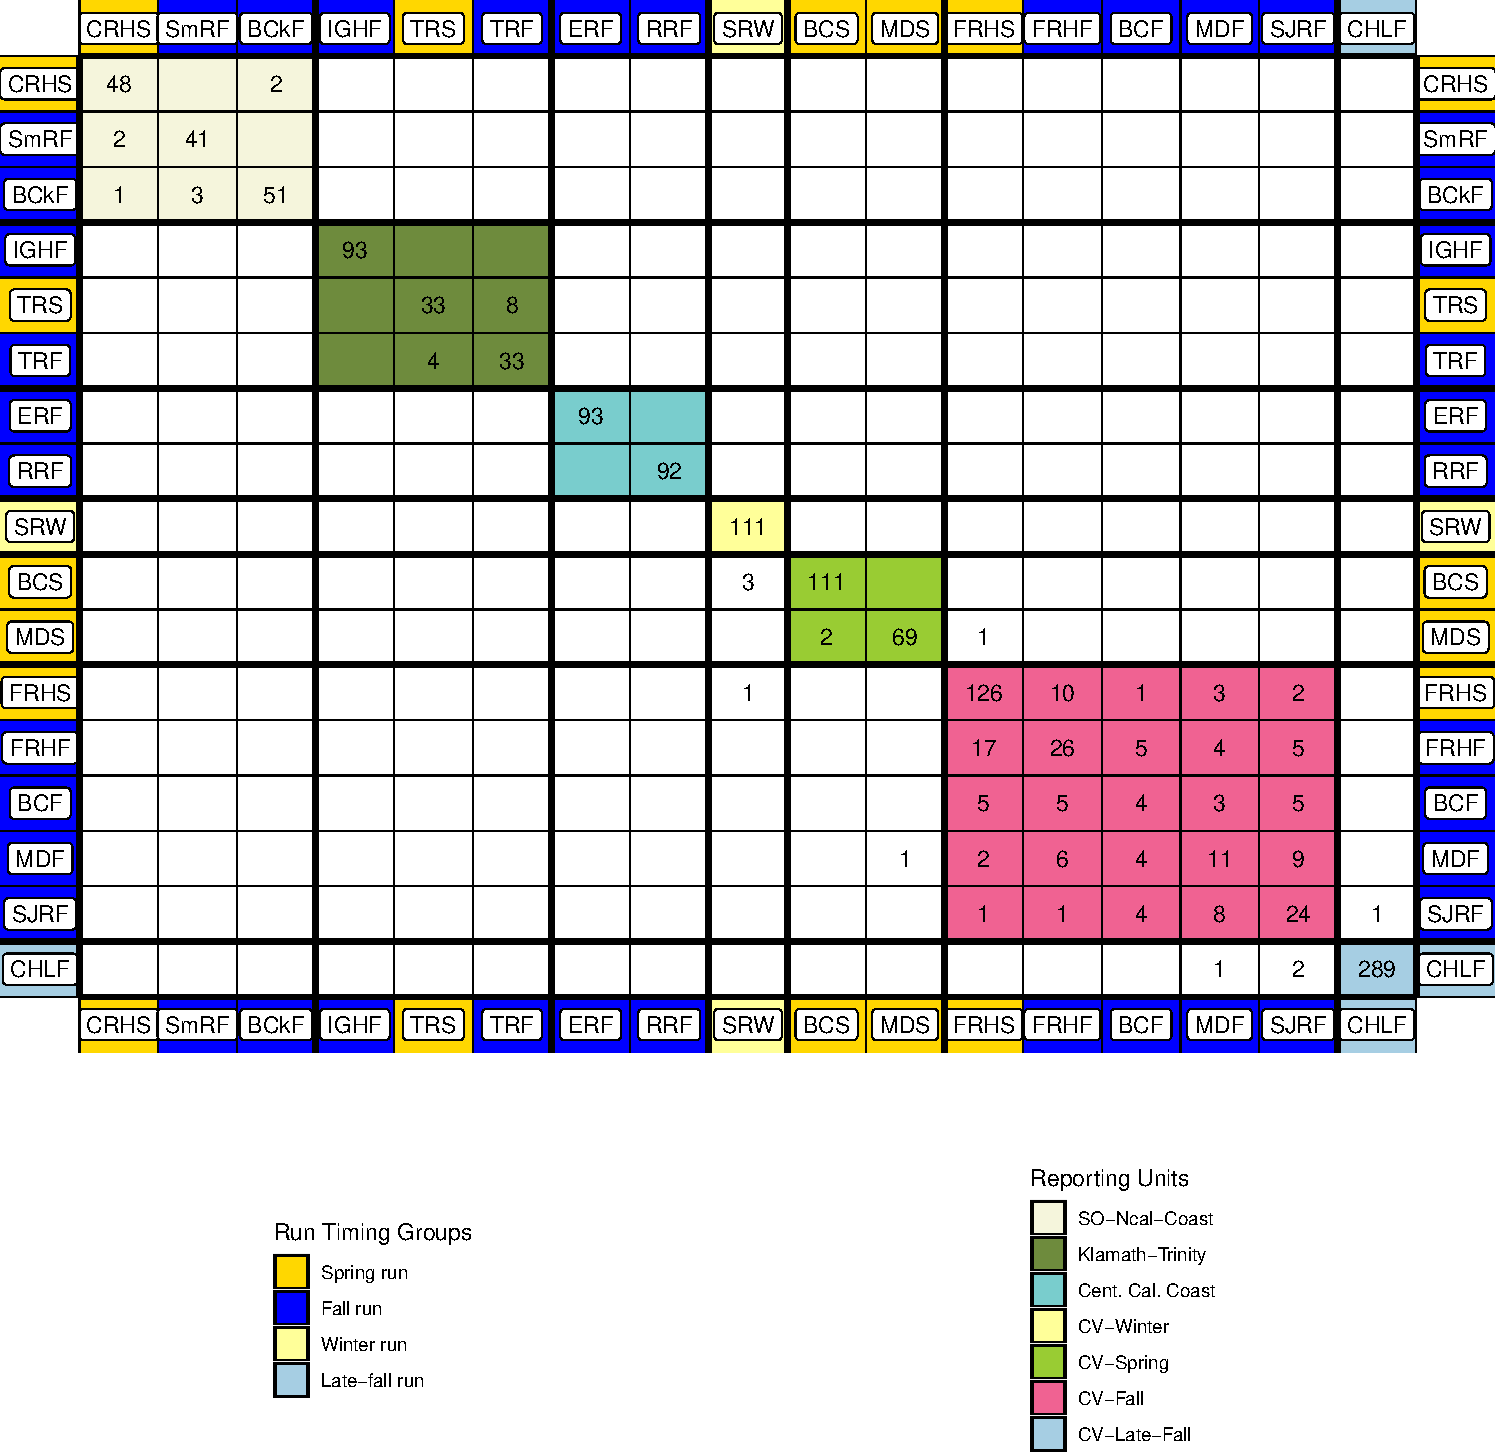
\includegraphics[width=0.8\textwidth]{images/ass-table-80-crop.pdf}
\end{center}
\caption[Assignment table for fish with scaled likelihood $ > 0.8$]{\footnotesize Assignment table
like that in Fig.~\ref{fig:gsi}b in the paper, but constrained so that only fish assigning
to a reporting unit with scaled likelihood greater than 0.8 are included.}
\label{fig:eighty}
\end{figure}
%%%%%%%%%%%%%%%%%%%%





%%%%%%%%%%%%%%%%%%%%%% 
\begin{figure}
\begin{center}
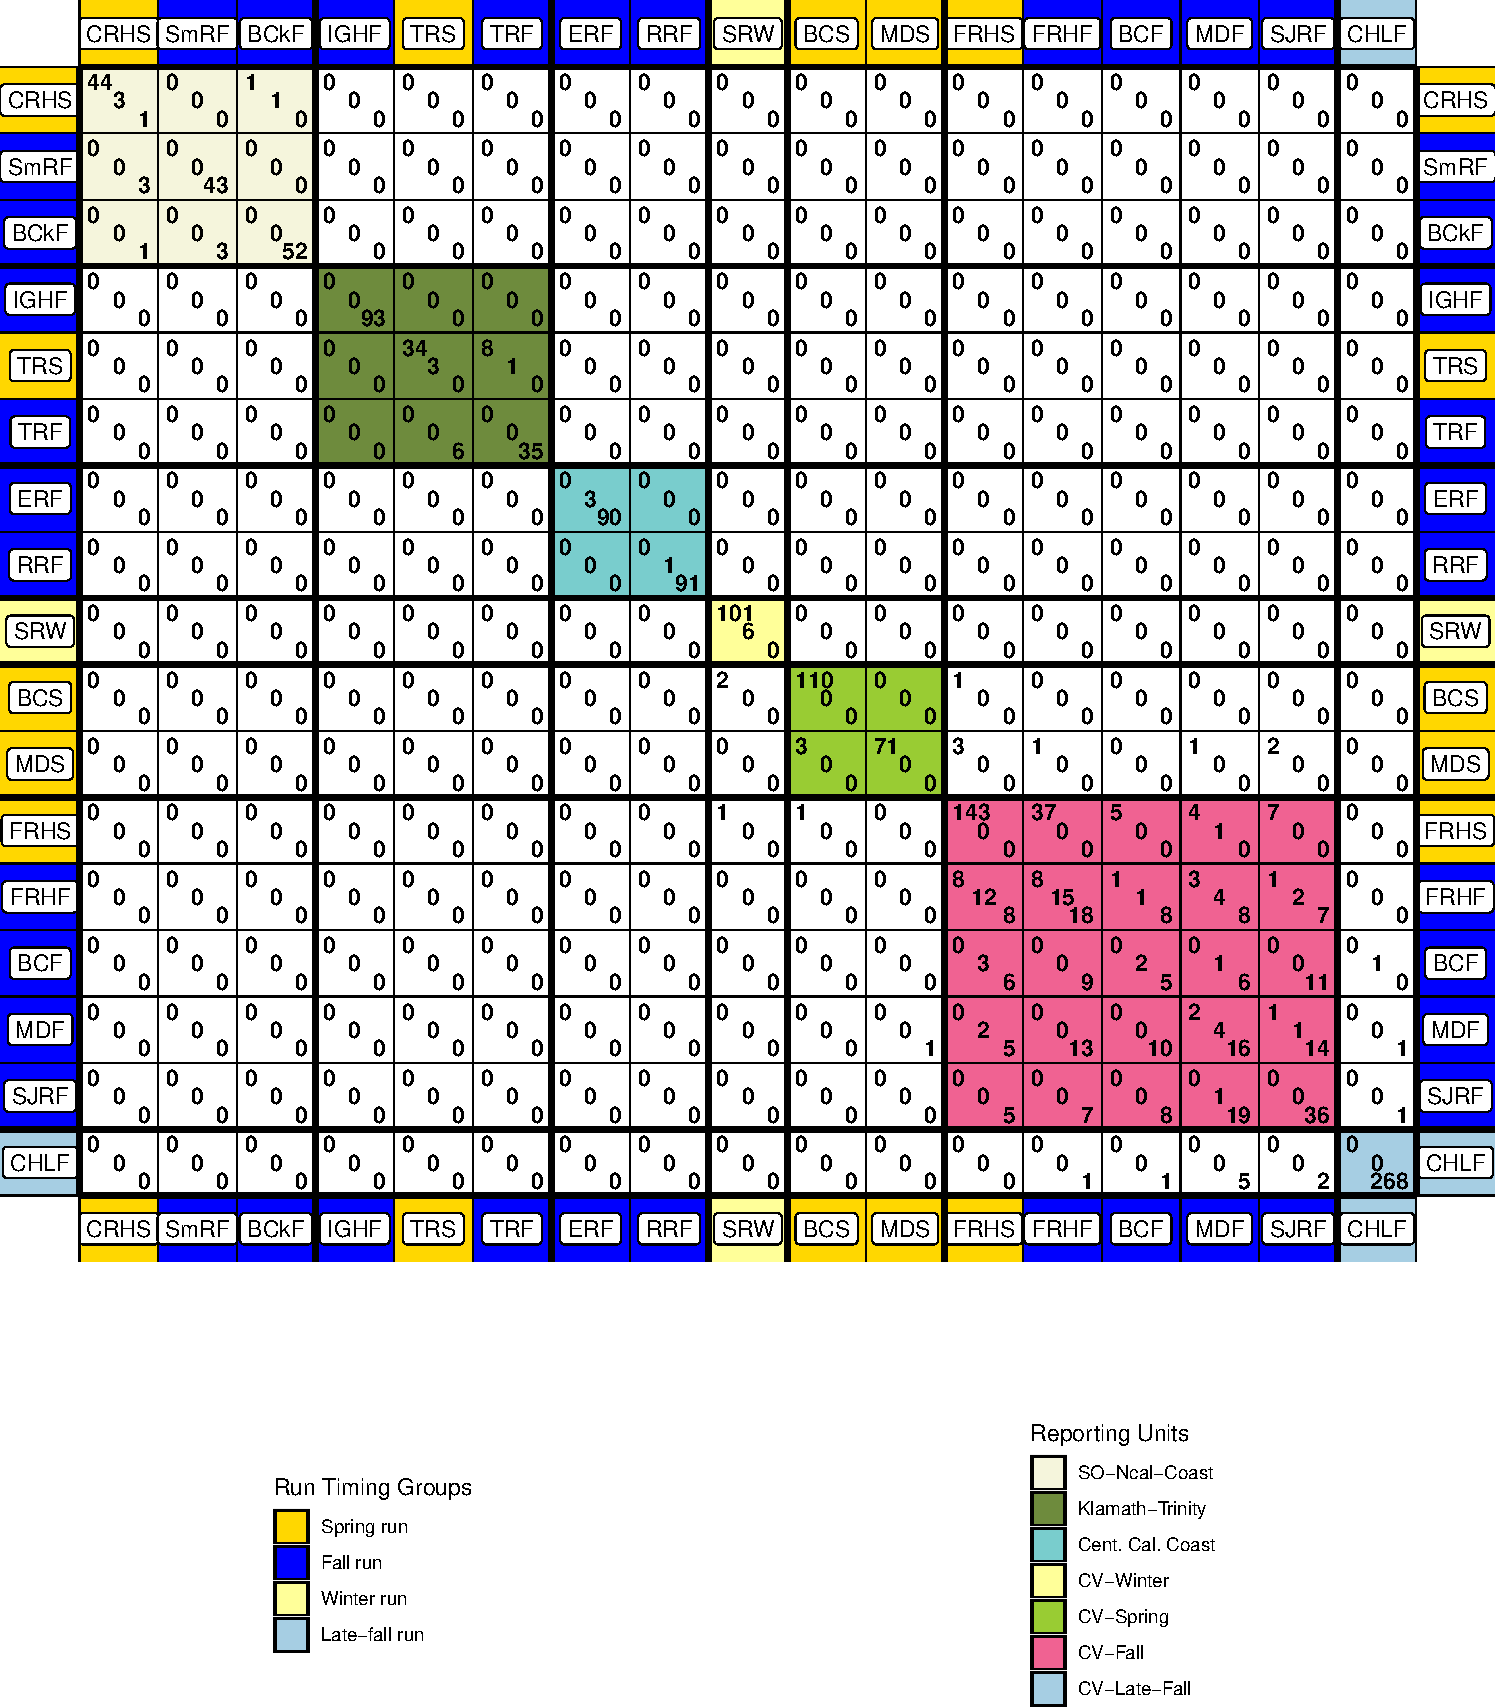
\includegraphics[width=0.8\textwidth]{images/rosa-gsi-table-crop.pdf}
\end{center}
\caption[Assignment table by RoSA genotype]{\footnotesize Assignment table
like that in Fig.~\ref{fig:gsi}b in the paper, but with numbers according to genotypes
at the RoSA. In each cell, the top left entry gives the number of EE (early run allele homozygotes)
genotypes, the middle entry is the number of EL genotypes (heterozygotes), and the bottom
right entry gives the number of LL (late-run homozygote) genotypes. }
\label{fig:rosa-gsi}
\end{figure}
%%%%%%%%%%%%%%%%%%%%



%%%%%%%%%%%%%%%%%%%%%% 
\begin{figure}
\begin{center}
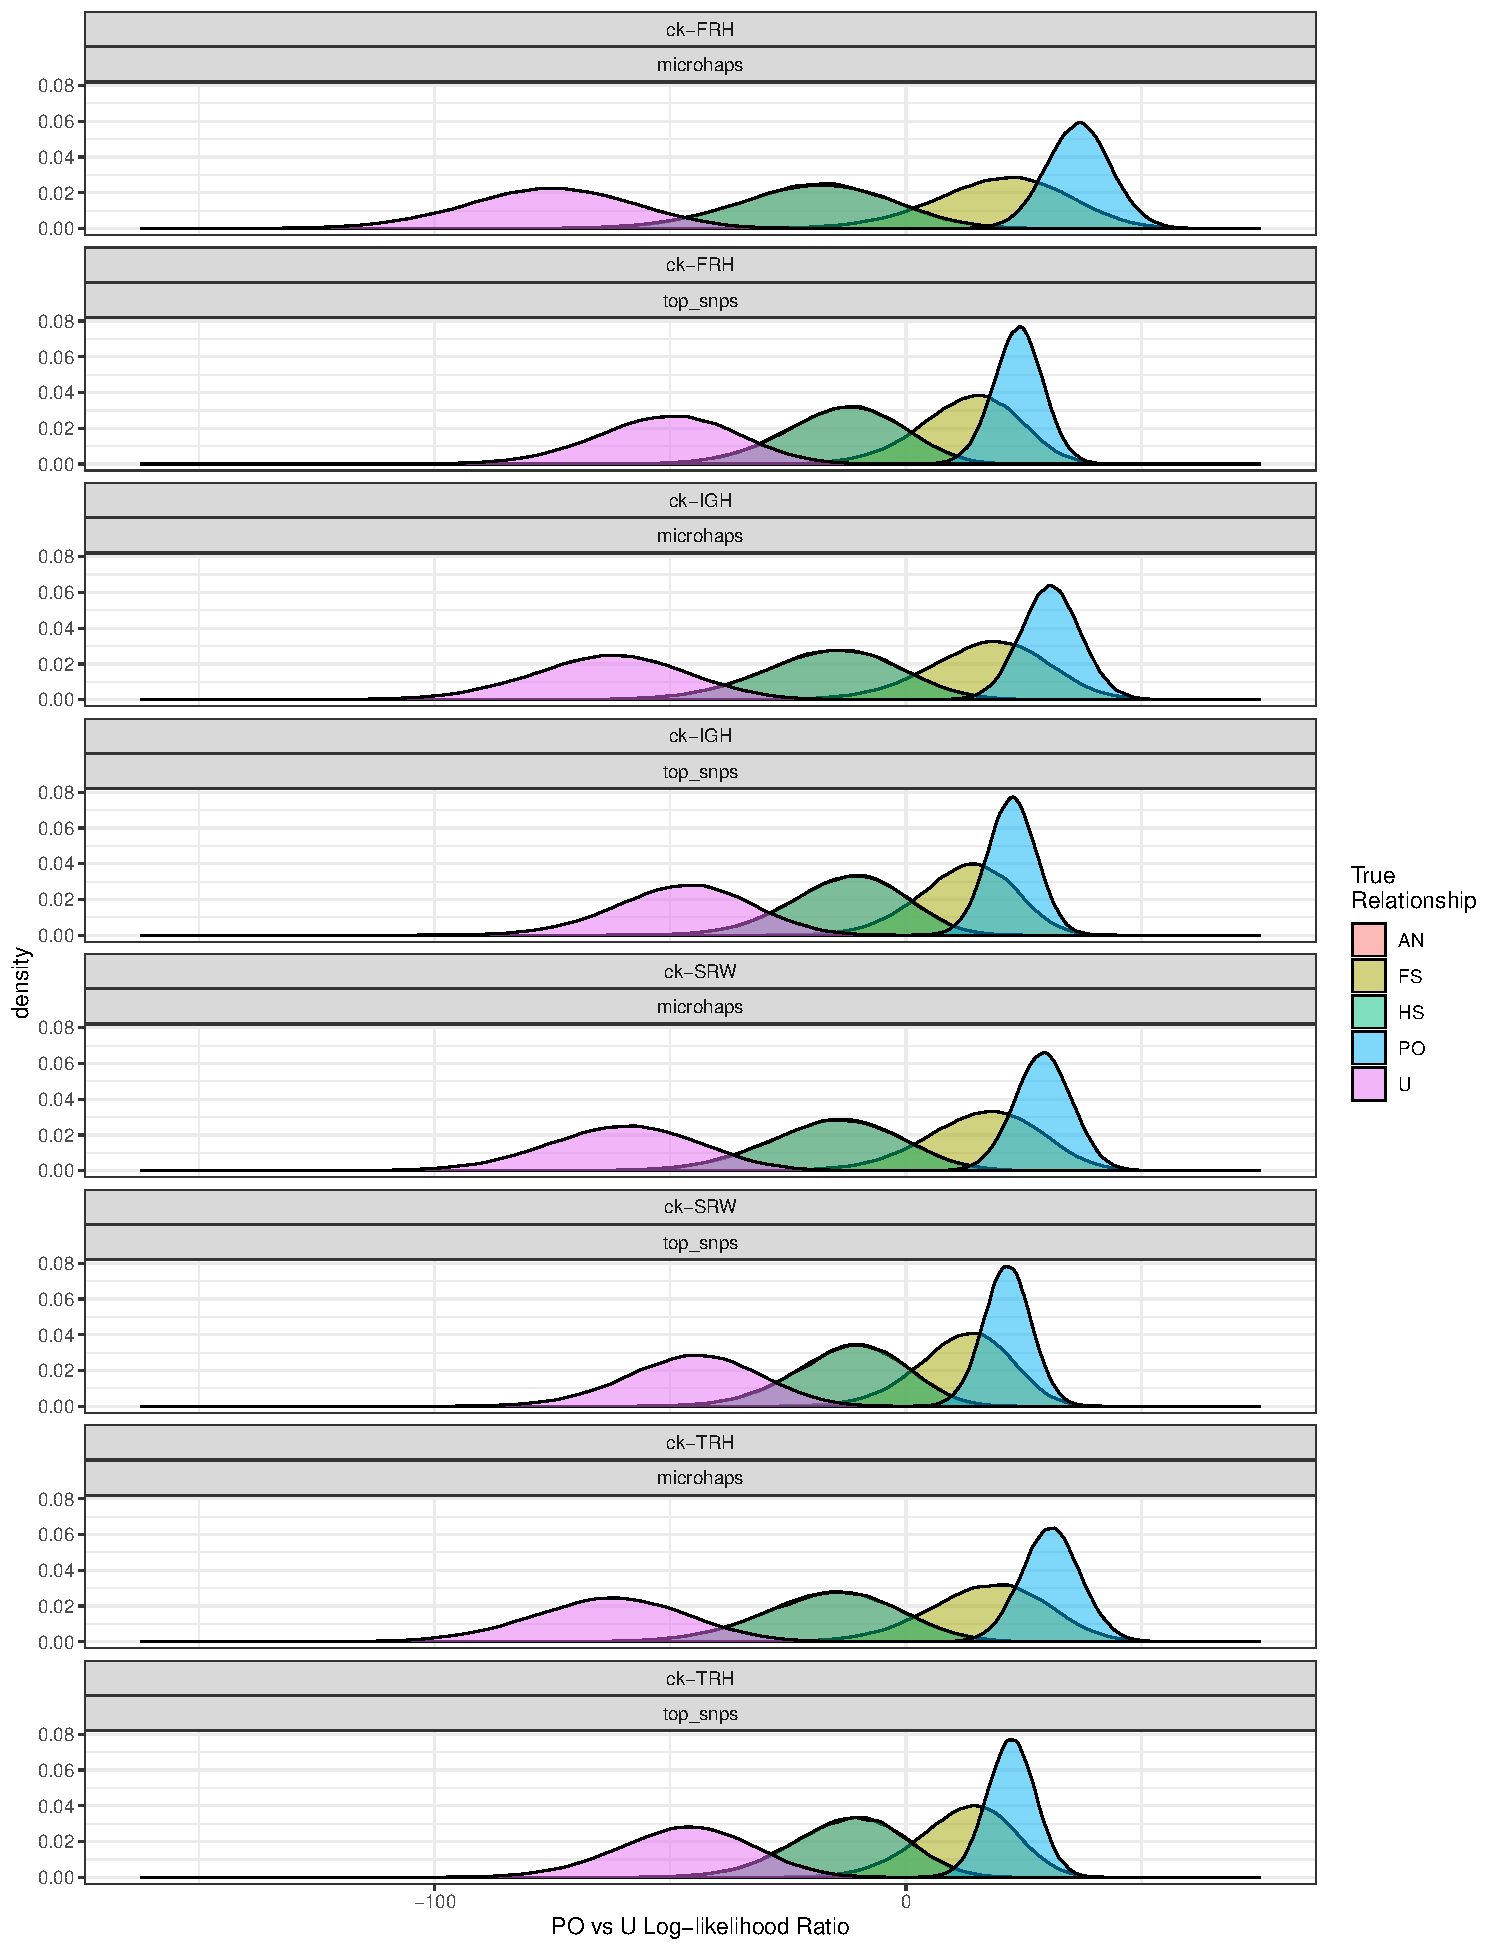
\includegraphics[width=0.9\textwidth]{images/cmkr-comp-figure-crop.pdf}
\end{center}
\caption[Comparison of microhaplotypes vs.~best SNP in each amplicon]{\footnotesize 
A comparison of the distribution of log-likelihood ratios when using all the alleles at each
amplicon typed as microhaplotypes ("microhaps" in the panel headers) versus using just a single (the most informative) SNP from each
amplicon ("top\_snps" in the panel headers).  Results shown for four hatchery collections in California 
(ck-FRH: Feather River Hatchery [spring and fall]; ck-IGH: Iron Gate Hatchery; ck-SRW: Sacramento Winter Run;
ck-TRH: Trinity River Hatchery [spring and fall]).  The density plots show
the distribution of log-likelihood ratios for Parent-Offspring vs Unrelated for four different relationships:
PO = parent offspring; FS = full-sibling; HS = Half sibling; AN = avuncular (i.e., aunt-niece, etc.)
The distributions for AN and HS overlap completely.  Note that the overlap between FS and PO occurs
for the PO vs U likelihood ratio, but is nearly eliminated with the PO vs FS likelihood ratio, allowing these
two relationships to be resolved accurately.}
\label{fig:ckmr-comp}
\end{figure}
%%%%%%%%%%%%%%%%%%%%

